\section{Introduction}
\label{sec:introduction}

Multi-party computation (MPC) allows $N$ parties $p_1,\dots, p_N$ to perform a computation on their private inputs securely. Informally, security means that the secure computation protocol computes the correct output (correctness) and it does not leak any information about the individual party inputs, other than what can be deduced from the output (privacy).

% The first results from the early 80's~\cite{FOCS:Yao82b,STOC:GolMicWig87,STOC:BenGolWig88,STOC:ChaCreDam88} introduced the problem and formally defined its security, and investigate feasibility in different models---e.g., passive or malicious adversaries, unconditional or computational security, with or without a broadcast channel. This spawned a rich theoretical literature of beautiful works improving and extending in various manners the original ideas.

MPC theory dates back to the early 1980-ies~\cite{Yao:1982,Goldreich:1987,Ben-Or:1988,Chaum:1988}.
Long the realm of theoretical cryptography, MPC has seen significant advances in programming technology in recent years.
These advances bring MPC closer to practice and wider applicability ---
MPC technology has been employed in real-world scenarios such as auctions~\cite{Bogetoft:2009}, biometric identification~\cite{Blanton:2011},
and privacy-preserving machine learning~\cite{Mohassel:2017,Mohassel:2018}.
The goal is to improve technology so that programmers can write \emph{secure} and \emph{efficient} programs without
commanding extensive knowledge of cryptographic primitives.

The problem, therefore, is to build a high-level programming language and a compiler, and there has been significant advance in
this space, e.g., ~\cite{Ben-David:2008,Bogdanov:2008,Zhang:2013,Hastings:2019,Keller:2020,Acay:2021,Braun:2022} among other work.
Current research largely falls at the two ends
of the classical compiler: (1) work on \emph{front-end} language design and (2) work on \emph{back-end} protocol implementation. Work on language design
focuses on high-level constructs necessary to express multiple parties, computation by different parties, and information flow from one party
to another~\cite{Rastogi:2014, Acay:2021}. On the other end, work on protocol implementation focuses on cryptographic foundations and their efficient circuit-level
implementation~\cite{Demmler:2015, Araki:2018, Braun:2022}, e.g., implementation of operations (e.g., MUL, ADD) using different sharing protocols
(Boolean or Arithmetic GMW~\cite{Goldreich:1987} or Yao's garbled circuits~\cite{Yao:1982}), as well as efficient share conversion from one representation
to another.

%Earlier compilers did both back-end and front-end translation as their aim was to demonstrate applicability of MPC on real-world
%programming problems. As the field advanced, works have focused more closely on front-end language design (e.g., Wysteria~\cite{SP:RasHamHic14} and Viaduct~\cite{Acay:2021})
%or back-end ``circuit-level'' design and implementation (e.g., MOTION~\cite{Braun:2022}).

In this work we focus on an intermediate language and what we call \emph{backend-independent optimizations}, in a close analogy to \emph{machine-independent} optimizations
in the classical compiler. The following figure summarizes our key idea:

{\begin{center}
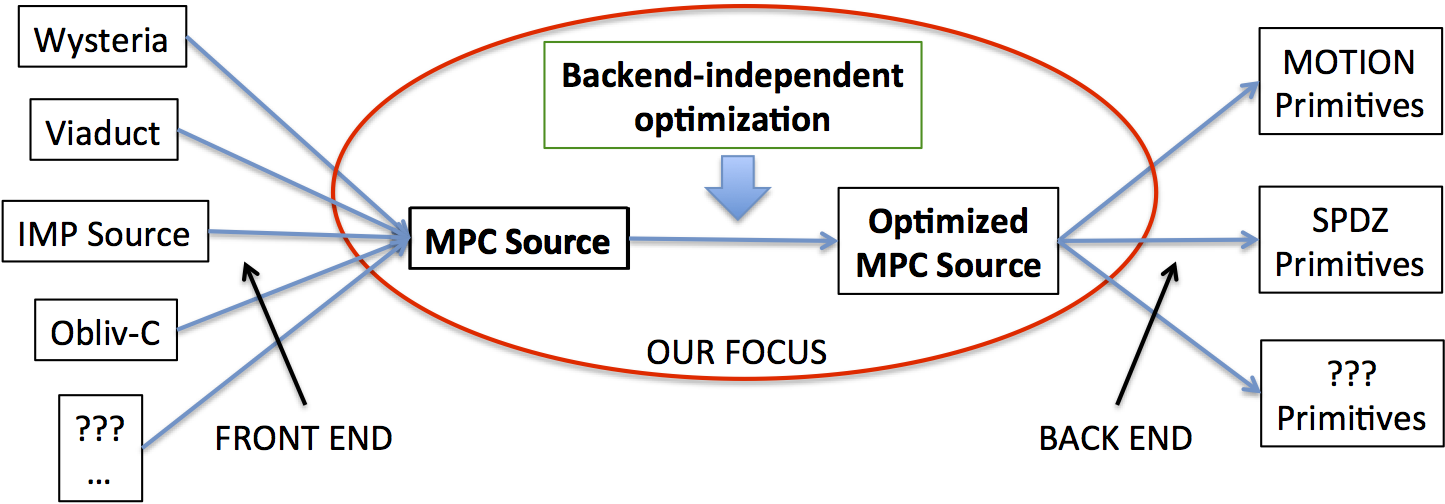
\includegraphics[width=0.8\linewidth]{figs_paper_SIMD/focus.png}
\end{center}
}

We formalize the MPC Source~\cite{Ishaq:2019} intermediate representation and emphasize optimization over MPC Source. As in classical compilers, we envision different front ends (e.g., our front end IMP Source) compiling into MPC Source. MPC Source is particularly suitable for optimizations such as protocol mixing~\cite{Buscher:2018b,Ishaq:2019, Fang:2022} and SIMD-vectorization,
which takes advantage of amortization at the circuit level. The MPC Source IR exposes the \emph{linear structure} of MPC programs, which simplifies program analysis; this is
in contrast to source, which has if-then-else constructs. In the same time, MPC Source is sufficiently ``high-level''  to support analysis and optimizations that take into account
control and data flow in a specific program. %MPC Source facilitates cost modeling. 
%MPC Source is small in size and analysis is tractable, as opposed to analysis over an unrolled circuit~\cite{Ishaq:2019}. 
Again as in classical compilers, we envision translation of MPC Source (optimized or unoptimized) into MOTION, SPDZ, or other back-end code.


%In contrast, the high-level program contains if-then-else and array writes, or the low-level circuit .
%The compilation problem, i.e., translation from a high-level language to circuits, is difficult and therefore, breaking the problem into sub-problems can  tractable.


\subsection{Our Contribution} In this paper, we develop a compiler framework that takes a Python-like routine and produces MOTION code. We describe: (a) the IMP Source language, its syntax and semantic restrictions, (b) translation into MPC Source, (c) a specific backend-independent optimization: novel SIMD-vectorization on MPC Source, and (d) translation from MPC Source into MOTION code. %\ana{I think we have to add more on MOTION, specifically mixing and amortization.}

We focus on the MOTION framework as our back-end for several reasons. First, it demonstrates high performance~\cite{Braun:2022}. Second, it provides an API over efficient implementation for a wide variety of cryptographic operations (e.g., MUL, CMP, etc.) in three different protocols ---  Arithmetic GMW, Boolean GMW, and BMR --- which allows for protocol mixing~\cite{Buscher:2018b,Ishaq:2019, Fang:2022}, a known backend-independent optimization. Third, MOTION provides API for SIMD-level operations (e.g., MUL\_SIMD), which amortize cost and lead to significant improvement in memory footprint and throughput~\cite{Demmler:2015, Araki:2018, Braun:2022}. It enables MPC Source-level vectorization, a key focus of this paper.

Our second contribution is an analytical model for cost estimation of amortized schedules. Originally, we hoped that optimal scheduling (under our model, which essentially minimizes the length of the schedule) was tractable, as the problem appeared simpler than the classical scheduling problem. Unfortunately, we show that optimal scheduling is NP-hard via a reduction to the Shortest Common Supersequence (SCS) problem. Cost modeling is important as it drives not only vectorization but optimizations such as protocol mixing and scheduling as well~\cite{Buscher:2018b,Ishaq:2019, Fang:2022}.

Our most important contribution is the implementation and evaluation of the compiler framework. We demonstrate expressivity of the source language by running the compiler on 16 programs with interleaved if- and for-statements; these include classical MPC benchmarks such as PSI and Biometric matching, as well as kMeans, Histogram, and other examples from the literature. 
Our compiler takes the routine and generated \emph{non-vectorized} MOTION code (from MPC Source on the picture above). It then optimizes MPC Source and generates 
\emph{vectorized} MOTION code (from Optimized MPC Source). We then run the two versions using Boolean GMW and the BMR protocols. (MOTION, which is designed for 
protocol mixing, supports Arithmetic GMW, however, it does not implement Comparison (CMP) and Multiplexing (MUX) as they would be rather inefficient.)
In our LAN experiments vectorized code exhibits 24x improvement on average in circuit generation time for Boolean GMW (20x for BMR), 7x reduction 
in communication (2x), 97x reduction in number of gates (91x), 4x improvement in setup time (23x) and 21x improvement in online time (18x).
%\ana{Summarize results.}

Our results emphasize the importance of backend-independent optimizations --- vectorization (described in this work) and protocol mixing (tackled in previous works~\cite{Buscher:2018b,Ishaq:2019, Fang:2022}) are two optimizations readily available at the level of MPC Source. We believe that our work can lead to future work on backend-independent compilation and optimization, ushering new MPC optimizations and combinations of optimizations in the vein of standard compilers, and thus bringing MPC programming technology closer to practice and wider applicability.

\subsection{Outline}

The rest of the paper is organized as follows. \secref{sec:overview} presents an overview of the compiler. \secref{sec:model} describes our model for cost estimation and argues NP-hardness of optimal scheduling. \secref{sec:compiler} details the front-end phases of the compiler, \secref{sec:vectorization} focuses in on backend-independent vectorization, and \secref{sec:backend} describes translation into MOTION. \secref{sec:results} presents the experimental evaluation.\secref{sec:related} discusses related work and \secref{sec:conclusion} concludes.

All our code, including benchmark Python-like code, compilation phases, and generated MOTION code is available on Github. We omit the link for anonymity, 
however, we will gladly make it available upon request from reviewers. The Github setup generates graphs and intermediate code for each benchmark along each compiler phase, it compiles with 
MOTION and runs the circuits on small inputs to generate tables of data (the experiments we present later run on real LAN and WAN). We plan to release the link and code, which we believe will be useful to researchers.

\begin{comment}
\begin{itemize}
\item We define the scheduling problem for MPC.
We present an analytical model to reason about cost of schedules
and show that scheduling is NP-hard via a reduction to the shortest
common supersequence problem.

\item We present a compiler that takes an IMP-like high-level
program and produces amortized (i.e., vectorized) low-level cryptographic
code in the MOTION framework. Central contributions are 1) a novel compiler framework,
2) a vectorization algorithm that produces optimal schedules for a large
number of MPC programs, and 3) reasoning over output arrays without Array SSA; we remove
infeasible loop-carried dependences introduced by standard SSA to improve vectorization.


\item We present an implementation and evaluation in the MOTION framework.
\ana{Fill in with final results. Mention benchmarks (standard + new ones + HyCC). }

\end{itemize}
\end{comment}
